\documentclass{standalone}

\usepackage[usenames,dvipsnames]{xcolor}
\usepackage{tikz}
\usepackage{pgfplots}
\usepackage{graphicx}
\usepackage{comment}

\pgfplotsset{compat=newest}

\definecolor{IBM1}{HTML}{648fff}
\definecolor{IBM2}{HTML}{785ef0}
\definecolor{IBM3}{HTML}{dc267f}
\definecolor{IBM4}{HTML}{fe6100}
\definecolor{IBM5}{HTML}{ffb000}
\definecolor{IBM6}{RGB}{051,117,056}

\definecolor{Okabe1}{RGB}{000,158,115}
\definecolor{Okabe2}{RGB}{000,114,178}
\definecolor{Okabe3}{RGB}{086,180,233}
\definecolor{Okabe4}{RGB}{230,159,000}
\definecolor{Okabe5}{RGB}{213,094,000}
\definecolor{Okabe6}{RGB}{204,121,167}

\begin{document}
	\vspace{1cm}
		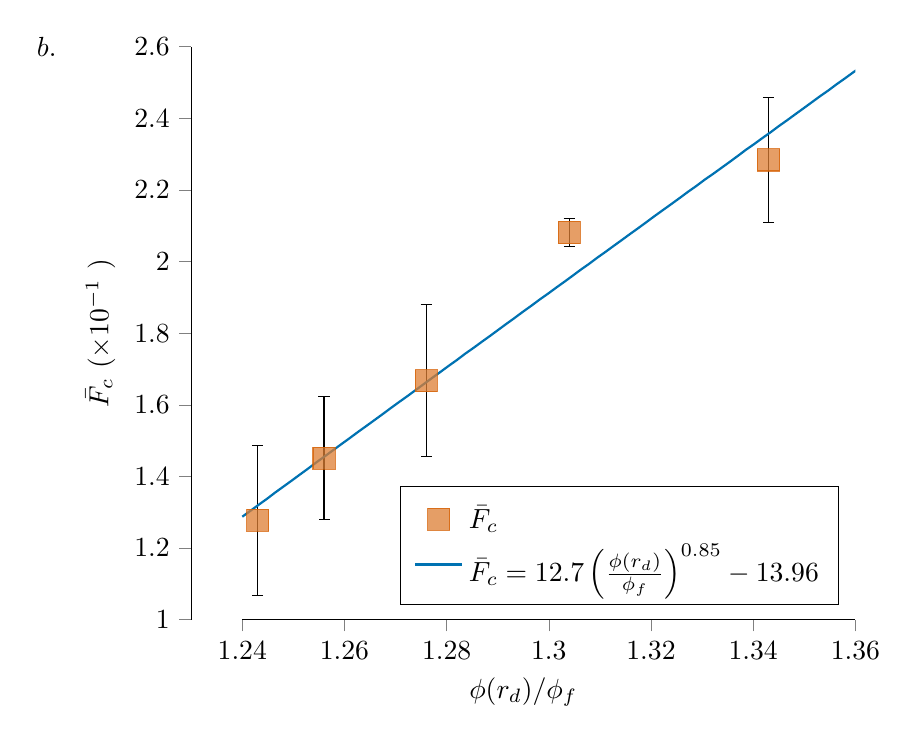
\begin{tikzpicture}
			\pgfplotsset{set layers}
		\begin{axis}[
			enlargelimits=false,
			title={$b.$},
			title style={yshift=-1ex, xshift=-5ex},
			tick pos=left, %
			tick align=outside, %
			axis line style={opacity=0}, %
			axis line style={opacity=0}, %
			after end axis/.code={
				\draw ({rel axis cs:0,0}
				-|{axis cs:1.24,0}) % xmin (line starts here)
				-- ({rel axis cs:0,0}
				-|{axis cs:1.36,0}); % xmax (line stops here)
				\draw ({rel axis cs:0,0}
				|-{axis cs:0,1}) % ymin (line starts here)
				-- ({rel axis cs:0,0}
				|-{axis cs:0,2.6}); % ymax (line stops here)
			},
			title={$b.$},
			title style={yshift=-2ex, xshift=-35ex},
			scale only axis,
			xmin=1.23, xmax=1.36,
			ymin=1, ymax=2.6,
			xlabel={$\phi(r_d)/\phi_f$},
			ylabel={$\bar{F}_{c}$ ($\times 10^{-1}$ )},
			legend style={at={(0.975,0.025)},anchor=south east,inner sep=5pt},
			scatter/classes={
				c={mark=square*,mark size=4pt,color=Okabe5,fill=Okabe5!80,opacity=0.75}
			}
			]
			\addplot[scatter,only marks,% 
			scatter src=explicit symbolic, % Needed for scatter class styling
			error bars/.cd,
			x dir=both, x explicit,
			y dir=both, y explicit
			] 
			table[y error index=2, meta=label] {
				x y yerr label
				1.243	1.277	0.209	c
				1.256	1.451	0.171	c
				1.276	1.667	0.212	c
				1.304	2.081	0.04	c
				1.343	2.284	0.174	c
			};

			\addplot[Okabe2, thick, domain=1.24:1.4, samples=100] {12.7*(x^0.85)-13.96};					
						
			\addlegendentry[anchor = west]{$\bar{F}_c$}

			\addlegendentry[anchor = west]{$\bar{F}_{c}=12.7\left(\frac{\phi(r_d)}{\phi_f}\right)^{0.85}-13.96$}
			
		\end{axis}
		
		
	\end{tikzpicture}

	
\end{document}